\documentclass[]{aa} %bibnumber

%\usepackage{hyperref}
\usepackage{txfonts}
\usepackage{amsmath, mathtools}
\usepackage[colorlinks,breaklinks]{hyperref}
\usepackage[normalem]{ulem}
\usepackage{cancel}
\hypersetup{linkcolor=blue,citecolor=blue,filecolor=black,urlcolor=blue}


\usepackage[dvipsnames]{xcolor}
\newcommand{\mr}[1]{{\textcolor[rgb]{0.60,0.10,0.6}{#1}}}
\newcommand{\mri}[1]{{\textcolor{red}{#1}}}
\newcommand{\nn}[1]{{\textcolor[rgb]{0.25, 0.50, 0}{#1}}}
\newcommand{\yc}[1]{{\textcolor{BrickRed}{#1}}}

\def\l{\lambda}\def\L{\Lambda}

\newcommand{\prob}[2]{\mathcal{P}\left( #1 \mid #2\right)}

\begin{document}
\title{Redshift Evolution of the Underlying Type Ia Supernova Stretch
Distribution}

\author{N. Nicolas
\thanks{n.nicolas@ipnl.in2p3.fr, equal contribution}
\inst{1}
    \and M. Rigault
    \thanks{m.rigault@ipnl.in2p3.fr, equal contribution}
    \inst{2}\and\\
    Y. Copin\inst{1}   
    \and R. Graziani\inst{2}
    %HERE ALPHABETIC ORDER
    \and G. Aldering\inst{3}
    \and M. Briday\inst{1}
    \and Y.-L. Kim\inst{1}
    \and Saul Perlmutter\inst{3}
    \and G. Smadja\inst{1}   
}

\institute{Université de Lyon, F-69622, Lyon, France; Université de Lyon
    1, Villeurbanne; CNRS/IN2P3, Institut de Physique des Deux Infinis, Lyon
    \and 
    Université Clermont Auvergne, CNRS/IN2P3, Laboratoire de
    Physique de Clermont, F-63000 Clermont-Ferrand, France.
    \and
    Physics Division, Lawrence Berkeley National Laboratory, 
    1 Cyclotron Road, Berkeley, CA, 94720 
}

\date{Received 2 November 1992 / Accepted 7 January 1993}

\abstract{
{The true nature of type Ia supernovae (SNe~Ia) remains largely unknown, and as
measure of survey statistic increase, the question of astrophysical systematic
uncertainties rises, and notably that of the SN~Ia population redshift drift.}
{In this paper, we study the redshift evolution of SN~Ia
\textsc{\texttt{SALT2.4}} lightcurve stretch\yc{\sout{es}}, \yc{\sout{which is}} a purely intrinsic SN
property, to probe this drift.}
{The SN stretch has been shown to strongly correlate with the SN's environment,
and notably with stellar age tracers. Following the \yc{evolution of} the fraction
of young and old SNe~Ia \yc{\sout{in nature} as predicted by} \cite{rigault2018}, and assuming
non-drifting \yc{$\to$constant/stationary?}  underlying stretch distribution for each \yc{population}, we model the expected
SN~Ia stretch distribution as a function of redshift. We test our prediction
against data from the literature chosen to have negligible selection
effects to ensure that any observed drift is indeed astrophysical and not
\yc{\sout{artificial} observational}.}
{We clearly demonstrate that the underlying SN\yc{e?}~Ia stretch distribution is
evolving as a function of redshift, and that the young/old drifting model is a
much better description of the data than any non-drifting model, including the
sample-based asymmetric distributions used by the Beams with Bias Correction
algorithm used to correct Malmquist bias. Our favored underlying stretch
model is bimodal: a high-stretch mode shared by both young and old environments,
and a low-stretch mode \yc{\sout{only existing in} exclusive to} old environments.}
{\sout{The underlying SNe~Ia population is evolving as a function of redshift \yc{This is purely a repetition of a previous sentence} \nn{\textit{see new sentence}} and the
exact impact on cosmology remains to be studied.} \nn{The precise impact of the redshift evolution of the underlying SNe Ia population on cosmology remains to be studied}. Yet, the astrophysical drift of
the SN stretch distribution does affect current Malmquist bias corrections and
thereby distances derived from SN affected by selection effects. We highlight
that such a bias will increase with surveys covering larger redshift ranges,
which is particularly important for LSST.}

}

\keywords{Cosmology -- Type Ia Supernova -- Systematic uncertainties}
\maketitle

\section{Introduction}

\yc{YC: you should run a grammar corrector, e.g. \texttt{grammarly}. e.g. "SNe dichotomy" vs. "SN dichotomy", "analysis" vs. "analyses", etc.}

Type Ia supernovae (SNe Ia) are powerful cosmological distance indicators that
have enabled the discovery of the acceleration of the Universe's expansion
\citep{riess1998, perlmutter1999}. They remain today a key cosmological probe to
understand the properties of dark energy (DE) as it is the only tool able to
precisely map the recent expansion rate ($z<0.5$), when DE is driving it
\citep[e.g.][]{scolnicastro2020}. They also are key to directly measure the
Hubble Constant (H$_0$), provided one can calibrate their absolute magnitude
\citep{riess2016, freedman2019}. Interestingly, the value of H$_0$ derived when
the SNe~Ia are anchored on Cepheids \citep[the SH0ES
project,][]{riess2009,riess2016} is $\sim5\sigma$ higher than what is predicted
\yc{from} cosmic microwave background (CMB) data measured by Planck assuming the
standard $\L$CDM \yc{ref?} \nn{textit{isn't it at the end of the sentence? Do you think it should be before the "or"?}}, or when the SN luminosity is anchored at intermediate
redshift by the baryon acoustic oscillation (BAO) scale
\citep{riess2019,reid2019,planck2018, feeney2019}. While using the tip of the
red giant branch technique in place of the Cepheids seem to favor an
intermediate value of H$_0$ \citep{freedman2019,freedman2020}, time delay
measurements from strong lensing seem to also favor high H$_0$ values
\citep{wong2019}.

The H$_0$ tension has received a lot of attention as it could be a sign of new
fundamental physics. Yet, no simple solution is able to accommodate this H$_0$
tension when accounting for all other probes \citep{knox2019} and the current
most promising scenario appears to be a burst of expansion at the
matter-radiation decoupling moment caused by a (fine tuned) early dark energy
\citep{poulin2019}. \yc{I don't see the point of going into this debate...}

Alternatively, systematic effects affecting one or several of the aforementioned
analyses could also explain the tension. \cite{rigault2015} suggested
that SNe Ia from the Cepheid calibrator sample differ by construction from the
Hubble flow \yc{ones} as it \yc{they?} strongly favors \yc{SNe don't favor anything...} \nn{\textit{but the Cepheid sample does, right?}} young stellar population environments where
one could find Cepheids. This selection effect would impact the derivation of
H$_0$ if SNe~Ia from young and older environments differ in average \yc{standardized} magnitudes. 

For the last decades, numerous analyses have studied the relation between SNe~Ia
and host properties, finding first that the standardized SNe~Ia magnitude
significantly depends on the host stellar mass, SNe~Ia from high-mass host being
brighter on average \cite[e.g.][]{kelly2010, sullivan2010, childress2013,
betoule2014, rigault2018, kim19}.  This mass-step correction is currently used
in cosmological analyses \citep[e.g.][]{betoule2014, scolnic2018a}, including
for deriving H$_0$ \citep{riess2016, riess2019}. Yet, the underlying connection
between the SNe and their host remains unclear when using global properties such as
the host stellar mass, which raises the question of the accuracy of the
correction. More recently, studies have used the local SN environment to probe
more direct connections between the SN and its environments \citep{rigault2013},
showing that local age tracers such as the local specific star formation rate or
the local color are more strongly correlated with the standardized SN magnitude
\citep{rigault2018, roman2018, kim18}, suggesting age as the driving parameter
underlying the mass-step. If true, this would have a significant impact for
cosmology because the redshift drift magnitude correction to apply might
strongly vary \yc{just the existence of a redshift-drift mag. correction is of importance here, even if it does not vary} \citep{rigault2013,childress2014,scolnic2018a}.  Yet, the
importance of local SN environmental studies remains highly debated
\cite[e.g.][]{jones2015,jones2019} and especially the impact it \yc{what does `it' refer to, the `importance'?} \nn{\textit{no, to the SN environment. Do you think it needs rephrasing?}} has on the
derivation of H$_0$ \citep{jones2015,riess2016,riess2018,rose2019}.

In this paper, we take a step aside to probe the validity of our modeling of the
SN population which we claim to be constituted of two age-populations
\citep{rigault2013,rigault2015,rigault2018}: one old and one younger, the former
having on average lower lightcurve stretches and being brighter after
standardization. We use the correlation between the SN age, \yc{as} probed by local
specific star formation rate \citep{rigault2018}, and the SN stretch to model
the expected evolution of the underlying SN stretch distribution as a function
of redshift. This modeling relies on three assumptions: (1) there are two
\yc{distinct} populations of SNe~Ia; (2) the relative fraction of each of these populations as
a function of redshift follows the \yc{model} presented in \cite{rigault2018}
and (3) the underlying distribution of stretch for each age sample \yc{is constant} \nn{\textit{what does it mean for a distribution to be constant? It seems weird that we say "does not significantly evolve" after saying it is constant, no?}} and does not significantly \yc{evolve with time}. This paper aims at testing this \yc{specific model} with
datasets from the literature.

\yc{Shouldn't this paragraph, introducing the concept of old and young populations and lsSFR, be moved \emph{before} the previous one?}
The concept of the SNe~Ia age dichotomy arose with the study of the SN~Ia rate.
\cite{mannucci2005, scannapieco2005, sullivan2006, aubourg2008} have shown that
the relative SNe~Ia rate in galaxies could be explained if two populations
existed, one young, following the host star formation activity, and one old
following the host stellar mass (the so called ``prompt and delayed'' or ``A+B''
model). In \cite{rigault2018} we used the specific Star Formation Rate at the SN
location (Local sSFR or LsSFR \yc{this has already been used multiple times, define before}) to classify which are the younger (those with a
high LsSFR) and which are the older (those with low LsSFR). Furthermore, since
the first SNe~Ia host analyses, the SN stretch has been known to be strongly
correlated with the SN host properties \citep{hamuy1996, hamuy2000}, which \yc{what does this ``which'' refer to?} has
been extensively confirmed since \citep[e.g.][]{neill2009, sullivan2010,
    lampeitl2010, kelly2010, gupta2011, dandrea2011, childress2013, rigault2013,
pan2014, kim19}. Following the ``A+B'' model and the connection between SN stretch
and host properties, \cite{howell2007} first discussed the potential redshift
drift of the SN stretch distribution. In this paper we revisit this analysis
with the most recent SNe~Ia dataset.

We present in section~\ref{sec:sample} the sample we are using for this
analysis, \yc{derived from} the Pantheon catalog \citep{scolnic2018a}. We
discuss the importance of obtaining a ``complete'' sample, i.e. representative of
the true underlying SNe Ia distribution, and how we build one from the Pantheon
sample. We then present in section~\ref{sec:modeling} our modeling of the
distribution of stretch as a function of redshift\nn{-}based models for the stretch
distribution of young and old SNe~Ia \yc{what??? rephrase} \nn{\textit{what isn't clear? Does the hyphen help?}}. Our results are presented in
section~\ref{sec:results}, where we test whether the SN stretch \yc{distribution} evolves as a
function of redshift and if the \yc{aforementioned} age model is in good agreement with this
evolution. Consequences for cosmology of our results are briefly discussed in
section~\ref{sec:bbc} and we conclude in section~\ref{sec:ccl}.

\section{Complete Sample Construction}\label{sec:sample}

We base our analysis on the \yc{most recent comprehensive} SNe~Ia compilation, the Pantheon catalog from
\cite{scolnic2018a}. A naive approach to test the SN stretch redshift drift
would be to simply compare the observed SN stretch distributions in a few bins
of redshift.  In practice, \yc{however}, \yc{differential} selection effects are affecting the observed SN
stretch distributions. Indeed, because the observed SN~Ia magnitude correlates
with the lightcurve stretch (and color), the first SNe~Ia that a
magnitude-limited survey will miss are the lowest-stretch (and reddest) ones.
Consequently, if \yc{magnitude-related} selection effects are not accounted for, one might confuse true
population drift with \yc{\sout{selection effects} survey properties}, and conversely.

Assuming sufficient (and unbiased) spectroscopic follow-up for acquiring typing
and host redshift, the selection effects of magnitude-limited surveys should be
negligible below a given redshift \yc{at which} even the faintest SNe~Ia can be observed.
In contrast, targeted surveys have highly complex selection functions and will
be discarded from our analysis. Fortunately, modern SN cosmology samples such as
the Pantheon \yc{one} are now dominated by magnitude-limited surveys.

We present in Fig.~\ref{fig:maglim} the lightcurve stretch and color of SNe~Ia from the following surveys: PanStarrs
\citep[PS1][]{rest2014}, the Sloan Digital Sky Survey
\citep[SDSS][]{frieman2008} and the SuperNovae Legacy Survey
\citep[SNLS][]{astier2006}. An ellipse in the \textsc{\texttt{SALT2.4}} $(x_1,
c)$ plane with $x_1 = \pm 3$ and $c = \pm 0.3$ encapsulates the full distribution
\citep{guy2007,betoule2014}; see also \citet{bazin2011} and \citet{campbell2013}
for similar contours, the second using a more conservative $|c| \leq 0.2$ cut.
Assuming the SN absolute magnitude with $x_1=0$ and $c=0$ is $M_0=-19.36$
\citep{kessler2009,scolnic2014}, we can derive the absolute standardized
magnitude at maximum of light $M = M_0 - \alpha x_1 + \beta c$ along the
aforementioned ellipse given the standardization coefficient $\alpha=0.156$ and
$\beta=3.14$ from \cite{scolnic2018a}: the faintest SN~Ia is that with
$(x_1=-1.66, c=0.25)$ and an absolute standardized magnitude at peak in Bessel $B$
band of $M^{t_0}_{min} = -18.31$~mag. Since one ought to detect this object
typically a week before and 10 days after peak to build a suitable lightcurve,
the \yc{effective} limiting standardized absolute magnitude is approximately
$M_{lim} = -18.00$~mag. Hence, given the magnitude limit $m_{lim}$ of a
magnitude limited survey, one can derive the maximum redshift $z_{lim}$ above
which the faintest SNe~Ia will be missed using the relation between apparent
magnitude, redshift and absolute magnitude $\mu(z_{lim}) = m_{lim} - M_{lim}$.

% YC: Figs and Tables *after* their 1st ref. in the text!
\begin{figure}
    \centering
    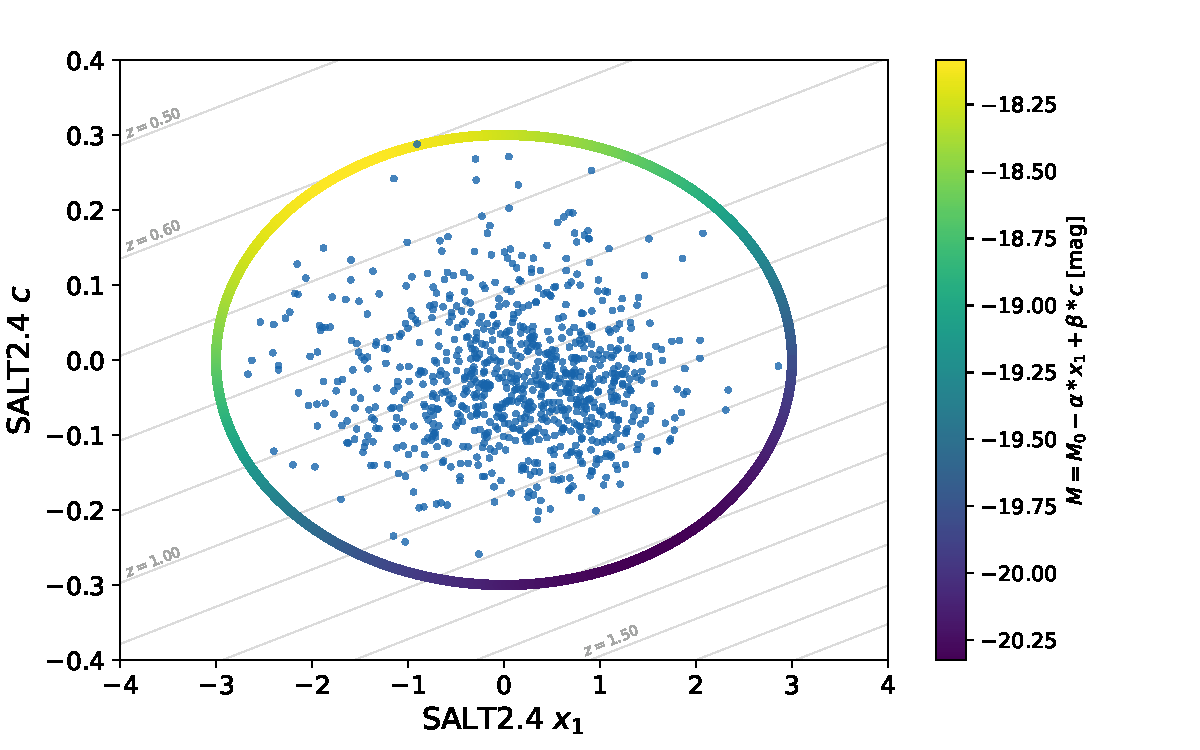
\includegraphics[width=0.95\linewidth]{Article_figures/zmax_maglim_snls.pdf}
    \caption{\textsc{\texttt{SALT2.4}} stretch ($x_1$) and color ($c$)
        lightcurve parameters of SNe~Ia from the SDSS, PS1 and SNLS samples of
        the Pantheon catalog.  The individual SNe are shown as blue dots and a
        2D histogram is shown in gray to highlight point density \yc{I don't think it's really needed}. The ellipse
        $(x_1=\pm3, c=\pm0.3)$ is displayed, colored by the corresponding
        standardized absolute magnitude using the $\alpha$ and $\beta$
        coefficients from \cite{scolnic2018a}. The grey diagonal lines represent
    the $(x_1, c)$ evolution for $m = m_{lim}$, for $z$ between $0.50$ and
$z=1.70$ using SNLS's $m_{lim}$ of $24.8$~mag.}
    \label{fig:maglim}
\end{figure}

SNLS typically acquires SNe~Ia in the redshift range $0.4<z<0.8$; at these
redshifts, the rest-frame Bessel $B$ band roughly corresponds to the SNLS $i$
filter, that has a $5\sigma$ depth of
24.8~mag\footnote{\href{https://www.cfht.hawaii.edu/Science/CFHTLS/cfhtlsfinalreleaseexecsummary.html}{CFHT
final release website.}}. This converts to a $z_{lim}=0.60$, in agreement with
\cite{neill2006}, \cite{perrett2010} and \cite{bazin2011}.  Fig.~14 of
\cite{perrett2010} suggests a lower limit of $z_{lim}=0.55$; both \yc{limits} will be
considered, as discussed below.

Similarly, PS1 observes SNe~Ia in the range $0.2<z<0.4$, their $g$-band
$5\sigma$ depth is 23.1~mag \citep{rest2014}, which yields to $z_{lim}=0.30$ in
agreement with, e.g., Fig.~6 of \cite{scolnic2018a}. This figure \yc{is also suggestive of} a more conservative $z_{lim}=0.27$.

In a similar redshift range, SDSS has a limiting magnitude of 22.5
\citep{dilday2008,sako2008}, which would lead to a $z_{lim}=0.24$. However, the
SDSS surveys were more sensitive to limited spectroscopic resources;
\cite{kessler2009} pointed out that during \yc{first} year of SDSS, SNe~Ia with
$r-mag<20.5$ were favored for spectroscopic follow-up, corresponding to a
redshift cut at $0.15$. For the rest of the SDSS survey, additional
spectroscopic resources were \yc{available}, and \cite{kessler2009} and \cite{dilday2008}
show a relative completeness \yc{what is a \emph{relative completeness}???} up to $z_{lim}=0.2$. Following these analyses, we
will use $z_{lim}=0.2$ as the baseline SDSS redshift limit.

For the rest of the analysis, we will consider the aforementioned redshift
limits, as well as more conservative \yc{values} for each of these surveys, namely
$z_{lim}=0.15$ for SDSS, $z_{lim}=0.27$ for PS1 and $z_{lim}=0.55$ for SNLS. \yc{why do you remind the conservative values, and not the fiducial ones? Just refer to Table~1.}

The complete sample selection is summarized in Table~\ref{tab:sample}, and the
redshift distribution of these three surveys are \yc{is?} shown in Fig.~\ref{fig:cuts}.
As expected, the selected redshift limits roughly correspond to the peak of
these histograms. 

\begin{table}
    \centering
    \caption{Composition of the SNe~Ia dataset used in this analysis.
    Conservative cuts are indicated in brackets.}
    \label{tab:sample}
    \begin{tabular}{l c c}
    \hline\hline%\\[-0.8em] % YC: don't, it's not your business to do that!
        Survey & $z_{lim}$ & $N_{\mathrm{SN}}$ \\%[0.15em]
        \hline%\\[-0.8em]
        SNf & -- & 114\\%[0.30em]
        SDSS & 0.20 (0.15) & 167 (82)\\%[0.30em]
        PS1 & 0.30 (0.27) & 160 (122)\\%[0.30em]        
        SNLS & 0.60 (0.55) & 102 (78)\\%[0.30em]
        HST & -- & 26\\%[0.30em]
        \hline%\\[-0.8em]
        Total & -- & 569 (422)\\%[0.30em]
        \hline
    \end{tabular}
\end{table}

\begin{figure}
    \centering
    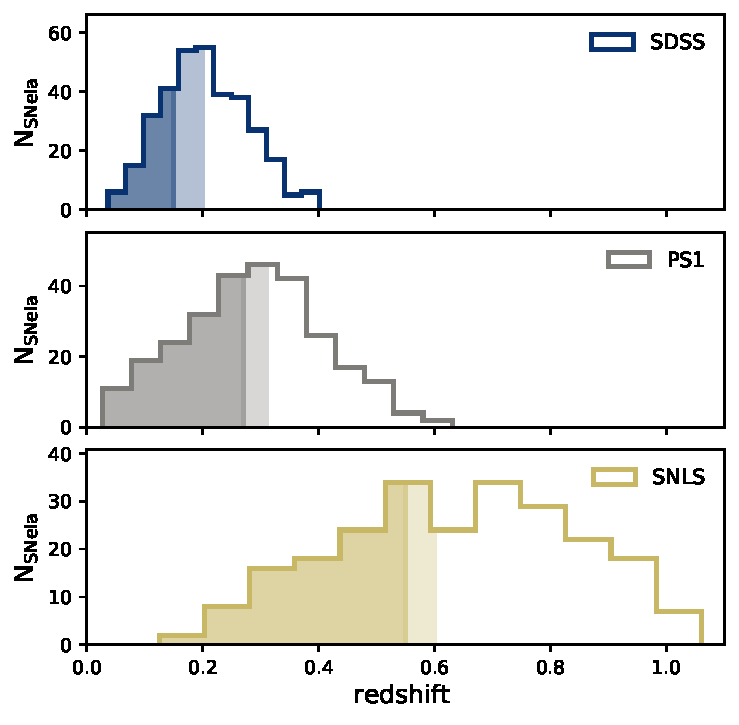
\includegraphics[width=0.95\linewidth]{Article_figures/hist_surveys_cuts_55-cividis.pdf}
    \caption{\textit{From top to bottom}: Redshift histograms of SNe~Ia from
        the SDSS, PS1 and SNLS dataset respectively (data from Pantheon,
        \citealt{scolnic2018a}).  The colored parts represent the distribution
        of SNe~Ia kept in our analysis for they are supposedly free from
        selection bias (see section~\ref{sec:sample}). The darker (resp. lighter)
    color responds to the conservative (resp. fiducial) selection cut.}
    \label{fig:cuts}
\end{figure}

In addition, we use the SNe~Ia from the Nearby Supernova Factory
\citep[SNfactory,][]{aldering2002} published in \cite{rigault2018} and that have
been discovered from non-targeted searches (114 SNe~Ia, see their sections~3 and~4.2.2; \mr{SNe~Ia time series are published in \citealt{Saunders2020}}). 
The spectroscopic follow-up was done over a redshift range of
$0.02<z<0.09$~\citep[as in ][]{rigault2018}, while the search was much
deeper. As such, these SNe~Ia \yc{\sout{should also} are assumed to} be a random sampling of the underlying
SN population. The SNfactory sample is particularly useful for studying SN property
drift, as it enables us to have a large SN~Ia sample at $z<0.1$.  

Finally, we include the HST sample from Pantheon, that \yc{\sout{follows the same logic
of having} similarly have} a search deeper than the follow-up and \yc{that} we therefore kept entirely
\citep{strolger04}. %, see Table~\ref{tab:sample}. 

We present the stretch
distribution and redshift histogram of these five surveys \yc{up to their respective $z_{lim}$} in
Fig.~\ref{fig:sample}.

\yc{You should also present/refer to Fig.5, showing the significant evolution of mean stretch as function of $z$ in complete samples. Next Sec. aims at modeling this evolution.}

\begin{figure}
    \centering
    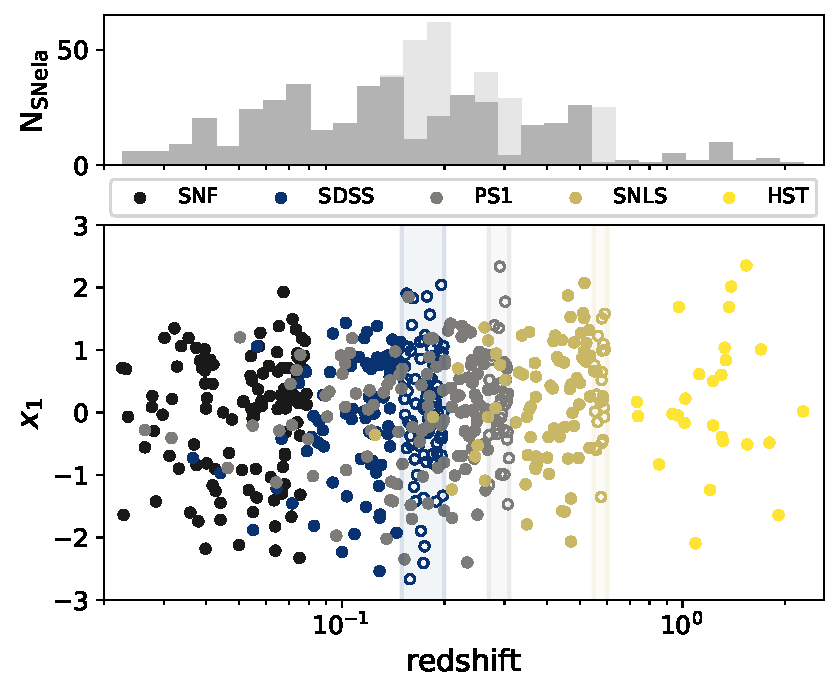
\includegraphics[width=0.95\linewidth]{Article_figures/stretchs-cut_btw_hist_cumu_75-lb-cividis.pdf}
    \caption{\textit{Bottom:} \textsc{\texttt{SALT2.4}} lightcurve stretch as a
        function of redshift for each survey considered in this
        analysis (see legend).  Solid (resp. open) markers correspond to the
        conservative (resp. fiducial) \yc{\sout{selection} redshift} cuts. \textit{Top:} combined
        redshift histogram in dark (resp. light) gray for the conservative
    (resp. fiducial) \yc{redshift} cuts.}
    \label{fig:sample}
\end{figure}

\section{Modeling the redshift drift}\label{sec:modeling}

\cite{rigault2018} presented a model for the evolution of the fraction of
younger vs. older SNe~Ia as a function of redshift following former work on
rates and delay time distributions \citep[e.g.,][]{mannucci2005,
scannapieco2005, sullivan2006, aubourg2008, childress2014, maozmannucci2014}.
In short, it was assumed that the number of \yc{``young''} SNe~Ia follows the star
formation activity (SFR \yc{R for activity? H for History?}) in the Universe, while the number of \yc{``old''} SNe~Ia
follows the number of Gyr-old stars in the Universe, i.e. the stellar mass
(M$^*$). Hence, if we denote $\delta(z)$ (resp. $\psi(z) = 1-\delta(z)$) the
fraction of young (resp. old) SNe~Ia in the Universe as a function of redshift,
then the ratio $\delta/\psi$ is expected to follow the evolution of the
specific star formation rate (SFR/M$^*$), which goes as $(1+z)^{2.8}$ until
$z\sim2$ \citep[e.g.,][]{tasca2015}. Since $\delta(0.05) \sim \psi(0.05)$
\citep{rigault2013,rigault2018,wiseman2020}, in agreement with rate expectations
\citep{mannucci2006,rodney2014}, \cite{rigault2018} concluded that
\begin{equation}
    \label{eq:delta}
    \delta(z) = \left( K^{-1} \times (1+z)^{-2.8} +1 \right)^{-1}
\end{equation}
with $K=0.87$. This model is comparable to the evolution predicted by
\cite{childress2014} based on SN rates in galaxies depending on their quenching
time as a function of their stellar mass.

\subsection{``Base'' underlying stretch distribution}
\label{sec:basemodel}

\yc{There is a generic confusion between ``SN stretch'' (individual SN, as in Eq.3/4) and something like ``SN stretch distribution'' (population, as in Eq.2). This is confusing...}

To model the evolution of the SN stretch \yc{distribution} as a function of redshift, given our
aforementioned model of the evolution of the fraction of younger and older
SNe~Ia with \yc{\sout{redshift} cosmic time}, we need to model the SN stretch distribution for each age
subsample. \yc{That paragraph sounds like a tautology...}

\yc{I suggest we remove the use of ``we'' when referring to previous papers, like ``In R+18, we did...'' to be replaced by ``R+18 did...''} 

\cite{rigault2018} presented the relation between SN stretch and LsSFR
measurement, \yc{a progenitor age tracer}, using the SNfactory sample. This
relation is shown in Fig.~\ref{fig:stretchlssfr} \yc{for SNf SNe used in the current analysis}. Given the structure of the
stretch-LsSFR scatter plot, our model of the underlying SN~Ia stretch
distribution is defined as follows:
\begin{itemize}
\item for the younger population (i.e., $\log(\mathrm{LsSFR})>-10.82$), the
\yc{\sout{underlying}} stretch distribution is modeled as a \yc{single} normal distribution
$\mathcal{N}(\mu_1, \sigma_1^2)$; 
\item the older population (i.e., $\log( \mathrm{LsSFR})<-10.82$) stretch
distribution is modeled as a \yc{bimodal} Gaussian mixture $a\times \mathcal{N}(\mu_1, \sigma_1^2) +
(1-a)\times \mathcal{N}(\mu_2, \sigma_2^2)$, 
where one mode is the same as for the young population, $a$
representing the relative influence of the two \yc{modes}.
\end{itemize}

\begin{figure*}
    \centering
    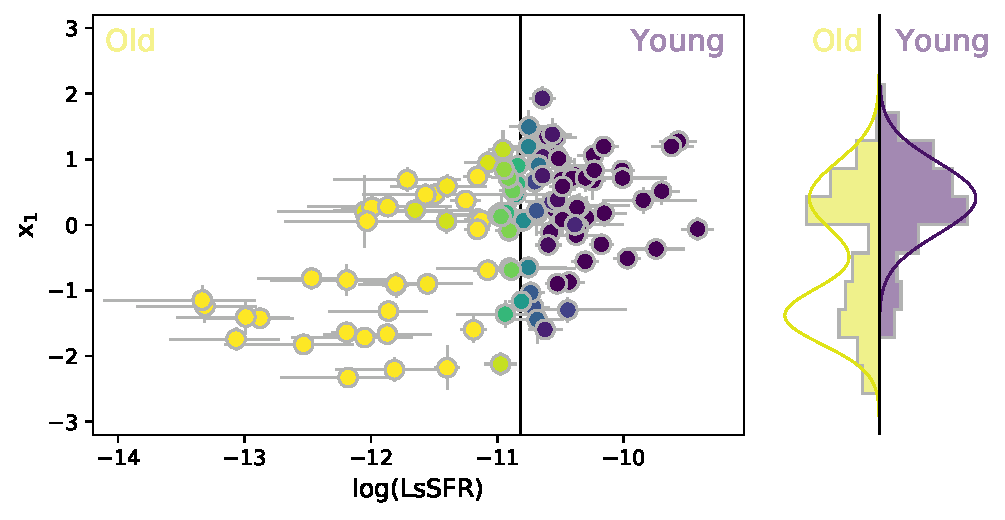
\includegraphics[width=0.8\linewidth]{Article_figures/model_base_hist.pdf}
    \caption{\textit{Main}: \textsc{\texttt{SALT2.4}} lightcurve stretch ($x_1$)
        as a function of the local specific star formation rate (LsSFR) for SNf
        SNe used in this analysis. The color corresponds to the probability,
        $p_y$, for the SNe~Ia to be young, i.e. to have $\log\mathrm{LsSFR} \geq
        -10.82$ \citep[see][]{rigault2018}. \textit{Right}: $p_y$-weighted histogram of the SN stretches, \yc{as well as the adjusted Base model}; the younger and
    older population contributions are shown in purple and yellow, respectively.}
    \label{fig:stretchlssfr}
\end{figure*}

When combined to the previously described prediction of the evolution of younger SNe~Ia as a function
of redshift (Eq.~\ref{eq:delta}), our model $X_1(z)$ for the underlying stretch distribution as a function of redshift is written
\begin{multline}
\label{eq:stretchz}
X_1(z) = 
\delta(z) \times \mathcal{N}(\mu_1,\sigma_1^2) + {} \\
(1 - \delta(z)) \times \left[a\times\mathcal{N}(\mu_1,\sigma_1^2) +
(1-a)\times\mathcal{N}(\mu_2,\sigma_2^2)\right].
\end{multline}
\yc{In fact, not clear what this eq. does here: it is supposed to be superseded by Eq.3/4. Maybe it should be moved to Sec.3.1.2 when we use $\delta(z)$ as a proxy to $y^i$.}

The maximum-likelihood estimate of the 5~free parameters
$\vec{\theta}\equiv({\mu_1,\mu_2,\sigma_1,\sigma_2,a})$ of the model is obtained by
minimizing the \yc{following} pseudo-$\chi^2$: %$\mathcal{X}^2$ defined as:
\begin{equation}
    \label{eq:likelihood}
    \mathcal{X}^2 = -2 \sum_i \ln \prob{x^{i}_{1}}{\vec{\theta};
    \mathrm{d}x^{i}_{1}, y^i},
\end{equation}
with
\begin{align}
    \label{eq:likelihoodsnf}
    \prob{x^{i}_{1}}{\vec{\theta}; \mathrm{d}x^{i}_{1}, y^i} =
    y^i &\times \mathcal{N}\left(x^{i}_{1} \mid \mu_1, \sigma_{1}^{2}+\mathrm{d}x^{i}_{1}{}^{2}\right) + {} \nonumber\\
        (1-y^i) &\times \bigg[
        a \times \mathcal{N}\left(x^{i}_{1} \mid \mu_1,
        \sigma_{1}^{2}+\mathrm{d}x^{i}_{1}{}^{2}\right) + {} \nonumber\\
     &(1-a) \times \mathcal{N}\left(x^{i}_{1} \mid \mu_2,
     \sigma_2{}^{2}+\mathrm{d}x^{i}_{1}{}^{2}\right) \bigg],
\end{align}
where $i$ is the index of the SN~Ia, $x^{i}_{1}$, $\mathrm{d}x^{i}_{1}$ and
$y^i$ are the \textsc{\texttt{SALT2.4}} stretch, its associated error and the
probability that the SN is young, respectively.  In practice, to ensure fraction
$a$ is constrained between 0 and 1, we fit for $\alpha$ such that
$a=\arctan(\alpha)/\pi+0.5$ \yc{\sout{, which results in an asymmetric error on $a$}}. \yc{Given the fact that 1. it's barely asymmetric ($a\sim 0.5$), 2. no one cares, it should be symmetrized (quadratically). Probably $\sigma$ errors are not symmetric either!}

Depending on whether $y^i$ can be estimated directly from LsSFR measurements or
not, there are two ways to proceed, which we now discuss.

\subsubsection{With LsSFR measurements}\label{sec:modelpy}

For the SNfactory sample, we can readily set $y^i = p_y{}^i$, the probability to
have $\log \mathrm{LsSFR} \geq -10.82$ (see Fig.~\ref{fig:stretchlssfr}), to
minimize Eq.~\ref{eq:likelihood} with respect to~$\vec{\theta}$.  Results on fitting
the SNf SNe with this model are shown Table~\ref{tab:modelresults} and
illustrated in Fig.~\ref{fig:stretchlssfr}.

\begin{table*}
    \centering
    \caption{Best fit values of the parameters for the Base stretch distribution
    model when applied to the SNfactory dataset only (114 SNe~Ia), the reference 569
SN~Ia sample or the conservative one (422).}
    \label{tab:modelresults}
    \begin{tabular}{lccccc}
    \hline\hline%\\[-0.8em]
        Sample & $\mu_1$  & $\sigma_1$ &$\mu_2$  & $\sigma_2$ & a \\%[0.15em]
        \hline%\\[-0.8em]
        SNfactory & $0.41 \pm 0.08$  & $0.55 \pm 0.06$ & $-1.38 \pm 0.10$ & $0.44 \pm 0.08$ & $0.48^{+0.08}_{-0.08}$ \\%[0.15em]
        Fiducial & $0.37 \pm 0.05$  & $0.61 \pm 0.04$ & $-1.22 \pm 0.16$ & $0.56 \pm 0.10$ & $0.51^{+0.09}_{-0.10}$ \\%[0.15em]
        Conservative & $0.38 \pm 0.05$  & $0.60 \pm 0.04$ & $-1.26 \pm 0.13$ & $0.53 \pm 0.08$ & $0.47^{+0.09}_{-0.08}$ \\%[0.15em]
        \hline
    \end{tabular}
\end{table*}

\subsubsection{Without LsSFR measurements}\label{sec:modelnopy}

When lacking direct LsSFR measurements (i.e. $p_y^i$), we can extend the
analysis to non-SNfactory samples by using the redshift-evolution of the
fraction $\delta(z)$ of young SNe~Ia (Eq.~\ref{eq:delta}) as a proxy for the
probability of a SN to be young. This still corresponds to minimizing
Eq.~\ref{eq:likelihood} with respect to the parameters $\vec{\theta}\equiv(\mu_1,
\mu_2, \sigma_1, \sigma_2, a)$ of the stretch distribution $X_1$
(Eq.~\ref{eq:stretchz}), but this time assuming $y^i = \delta(z^i)$ for any
given SN~$i$. 

For the rest of the analysis, we will therefore minimize Eq.~\ref{eq:likelihood}
using $p_y{}^i$ --~the probability for the SN $i$ to be young~-- when available
(i.e. for SNfactory dataset), and $\delta(z^{i})$ --~the expected fraction of
young SNe~Ia at the SN redshift $z^{i}$~-- otherwise.

Results of fitting this model to all the 569 (resp. 422) SNe from the fiducial
(resp. conservative) sample are given Table~\ref{tab:modelresults} and
\yc{predicted redshift evolution of mean stretch} illustrated in Fig.~\ref{fig:modelall}. \yc{I'm confused: grey points in Fig.5 are model independent, aren't they? Only the curve is related to the model.} We see in this figure that the measured
mean SN~Ia stretch per bin of redshift closely follows our redshift drift
modeling; that is, when considering selection-bias-free SN~Ia samples, SNe~Ia at
higher redshift have on average larger stretch ($0.34 \pm 0.10$ at $z\sim0.65$)
than those at lower redshift ($-0.17\pm 0.10$ at $z\sim0.05$). \yc{This is model-independant, and a nice result by itself, and should be already mentioned right at the end of Sec.2.}  This is indeed
what is expected if old environments favor low SN stretches
\citep[e.g.][]{howell2007} \emph{and} if the fraction of old SNe~Ia declines as
a function of redshift. See section~\ref{sec:results} for a more quantitative
discussion.

\begin{figure*}
    \centering
    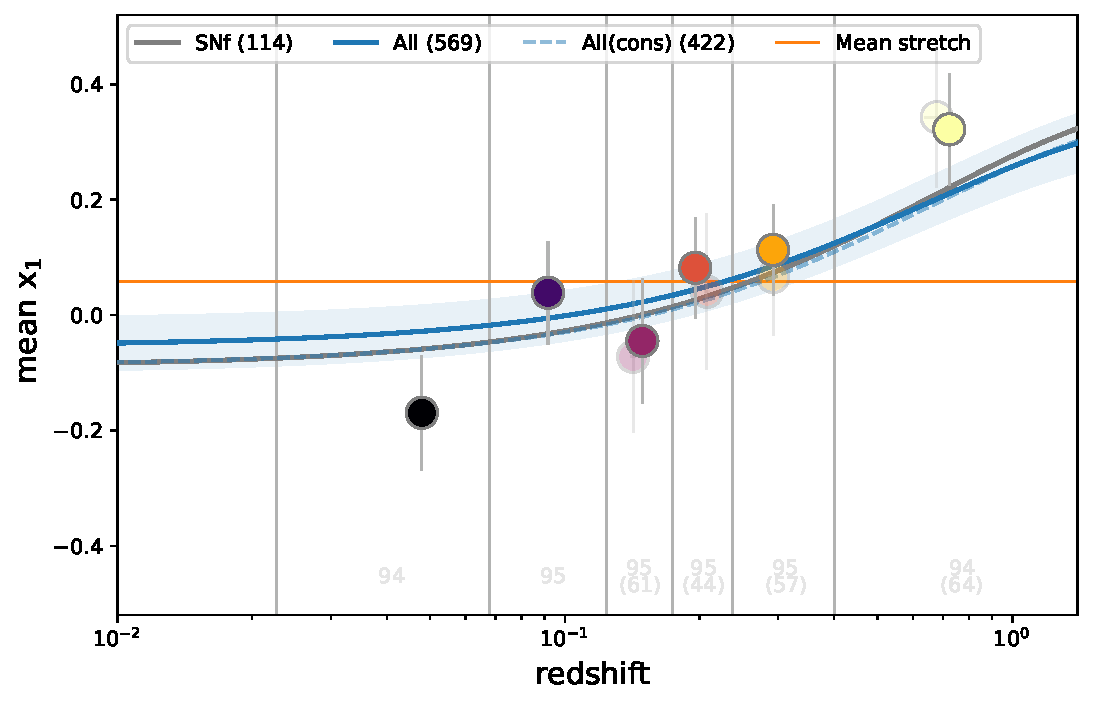
\includegraphics[width=0.7\linewidth]{Article_figures/stretchevol_all_vs_snf.pdf}
    \caption{Evolution of the mean SN \textsc{\texttt{SALT2.4}} stretch ($x_1$)
        as a function of redshift. Markers show the mean stretch measured in
        redshift bins of equal sample size, indicated in light gray at the
        bottom of each redshift bins. Full and light markers are used when
        considering the fiducial or the conservative samples, respectively. The
        orange horizontal line represents the mean stretch of the reference
        sample, illustrating the expectation if the SN stretch distribution is
        not evolving with redshift. Best fits of our Base drifting model are
        shown as blue, dashed-blue and gray, when fitted on the fiducial sample,
        the conservative one or the SNfactory dataset only, respectively; all
        are compatible. The light-blue band illustrates the amplitude of the
    error of the best fit model when considering the reference dataset.}
    \label{fig:modelall}
\end{figure*}

\subsection{Alternative models}\label{sec:othermodel}

In section~\ref{sec:basemodel}, we have modeled the underlying stretch
distribution following \cite{rigault2018}, i.e.\ as a single Gaussian for the
``young'' SNe~Ia and a mixture of two Gaussians for the ``old'' SNe Ia population, one
\yc{being} the same as for the young population, plus another one for the fast-declining SNe~Ia
that seem to only exist in old \yc{\sout{host galaxy stellar populations} local environments}.
This is our so-called ``Base'' model.
However, to test different modeling choices, we have implemented a suite of
alternative parametrizations that we also adjust to the data following the
procedure described in section~\ref{sec:modelnopy}. 

\cite{howell2007} used a simpler \yc{unimodal} model per age category, assuming a \yc{single} normal
distribution for \yc{each of} the young and old populations. We thus consider a
``Howell+drift'' model, with one single Gaussian per age group and the
$\delta(z)$ drift from Eq.~\ref{eq:delta}.

Alternatively, since we aim at probing the existence of an \yc{evolution with redshift}, we
also test \yc{constant} models by restricting the ``Base'' and ``Howell'' models
to use a supposedly redshift-independent fraction $\delta(z) \equiv f$ of young SNe;
these models are \yc{hereafter} labeled ``Base+constant'' and ``Howell+constant''.

We also consider another \yc{intrinsically} non-drifting model, the one developed for Beams
with Bias Correction \cite[BBC,][]{scolnic2016, kessler2017}, used in recent SN
cosmological analyses \cite[e.g.][]{scolnic2018a, descosmopaper2019, riess2016,
riess2019} to account for Malmquist biases. The BBC formalism assumes
sample-based (hence intrinsically non-drifting) asymmetric Gaussian stretch
distributions: $\mathcal{N}\left(\mu,
\sigma_{-}^2\;\text{if}\;x_1<\mu,\;\text{else}\;\sigma_{+}^2\right)$. The idea
behind this sample-based approach is twofold: (1) Malmquist biases are driven by
survey properties and (2) \yc{since} current surveys cover limited redshift ranges,
doing so \yc{what?} covers some potential redshift evolution information
\citep{scolnic2016, scolnic2018a}. See further discussion concerning BBC in
section~\ref{sec:bbc}. 

Finally, for the sake of completeness, we also consider simple the ``Gaussian'' and
``Asymmetric'' Gaussian non-drifting models. 

\section{Results}\label{sec:results}

We \yc{adjusted} each of the models described above on both the reference and conservative samples (cf.
section~\ref{sec:sample}); \yc{results are gathered in Table~\ref{tab:comp}, and illustrated in Fig.~\ref{fig:mod_comp}.} 

\yc{Since} the \yc{various} models have different degrees of freedom, we use the Akaike
Information Criterion \citep[AIC, e.g.][]{burnham2004} to compare \yc{their ability to properly describe the observations}. This
estimator penalizes extra degrees of freedom to avoid over-fitting the data, and
is defined as follow:
\begin{equation}
    \mathrm{AIC} = \mathcal{X}^2_{min} + 2k
\end{equation}
where $\mathcal{X}^2_{min}$ is the minimum value of the pseudo-$\chi^2$ as
defined Eq.~\eqref{eq:likelihood}, and $k$ is the number of free parameters \yc{to be adjusted}. The
reference model is the one with the smallest AIC; in comparison to this model,
the models with $\Delta\mathrm{AIC}<5$ are \yc{coined} acceptable, the ones with
$5<\Delta\mathrm{AIC}<20$ are unfavored, and those with $\Delta\mathrm{AIC}>20$
are \yc{deemed} excluded. This roughly corresponds to 2, 3 and 5~$\sigma$ limits for a
Gaussian probability distribution.

\begin{table*}
\centering
\caption{Comparison of the relative ability for a model to describe the
data. For each considered model, we report if the model is drifting or not,
its number of free parameters and, for both the fiducial and the conservative
cuts, the pseudo-$\chi^2$, $\mathcal{X}^2$ (see Eq.~\ref{eq:likelihood}), the AIC
and the AIC difference ($\Delta$AIC) between this model and the Base model used
as reference for it has the lowest AIC.}
    \label{tab:comp}
    \begin{tabular}{ccc|ccc|ccc}
    \hline\hline%\\[-0.8em]
        & & & \multicolumn{3}{c}{Fiducial sample (569 SNe)} & \multicolumn{3}{|c}{Conservative sample (422 SNe)} \\
        %\cline{2-6}
        Name & drift & $k$ &
        $\mathcal{X}^2$ & AIC & $\Delta \mathrm{AIC}$ & $\mathcal{X}^2$ & $\mathrm{AIC}$ & $\Delta \mathrm{AIC}$\\%[0.15em]
        \hline%\\[-0.8em]

        Base & $\delta(z)$ & 5
        & 1456.7 & 1466.7 & -- 
        & 1079.5 & 1089.5 & -- \\%[0.15em]

        Howell+drift & $\delta(z)$ & 4
        & 1463.3 & 1471.3 & $-4.6$  %&$1.0\times10^{-1}$
        & 1088.2 & 1096.2 & $-6.7$ 
        %& $3.4\times10^{-2}$
        \\%[0.15em]

        Asymmetric & -- & 3
        & 1485.2 & 1491.2 & $-24.5$  %&$4.7\times10^{-6}$
        & 1101.3 & 1107.3 & $-17.8$ 
        %& $1.4\times10^{-4}$
        \\%[0.15em]

        Howell+const & $f$ & 5
        & 1484.2 & 1494.2 & $-27.5$  %&$1.0\times10^{-6}$
        & 1101.2 & 1111.2 & $-21.7$ 
        %& $1.9\times10^{-5}$
        \\%[0.15em]

        Base+const & $f$ & 6
        & 1484.2 & 1496.2 & $-29.5$  %&$3.9\times10^{-7}$
        & 1101.2 & 1113.2 & $-23.7$ 
        %& $7.1\times10^{-6}$
        \\%[0.15em]

        \yc{BBC-like?} & per sample & 3x5
        & 1468.2 & 1498.2 & $-31.5$  %&$1.5\times10^{-7}$
        & 1083.6 & 1113.6 & $-24.1$ 
        %& $5.7\times10^{-6}$
        \\%[0.15em]

        Gaussian & -- & 2
        & 1521.8 & 1525.8 & $-59.1$  %&$1.5\times10^{-13}$
        & 1142.6 & 1146.6 & $-57.1$ 
        %& $4.0\times10^{-13}$ 
        \\
        \hline
    \end{tabular}
\end{table*}

\begin{figure}
    \centering
    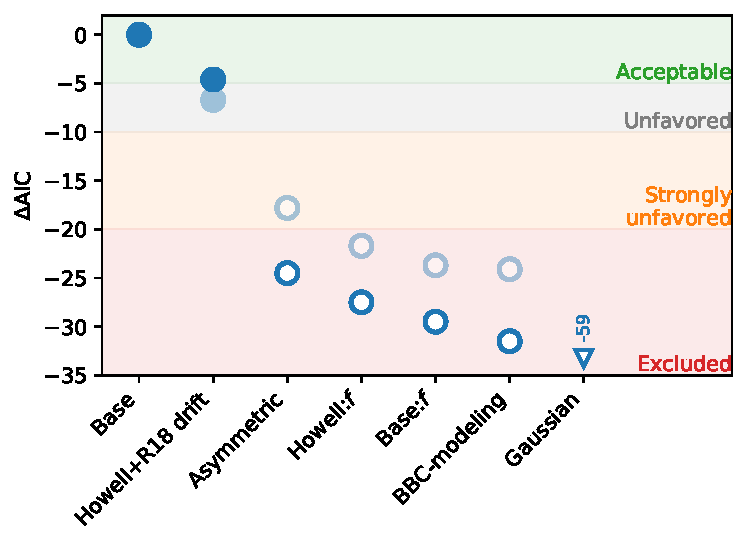
\includegraphics[width=\linewidth]{Article_figures/mod_comp.pdf}
    \caption{$\Delta$AIC between ``Base'' model (reference) and other models
        (see Table~\ref{tab:comp}). Full and open blue markers correspond to
        models with and without redshift drift, respectively. Light markers show
        the results when the analysis is performed on the conservative sample
        rather than the fiducial one.  Color-bands illustrate the validity of
        the models, from  Acceptable ($\Delta\mathrm{AIC} > -5$) to Excluded
        ($\Delta\mathrm{AIC} < -20$), see text. According to the AIC, all
    non-drifting models (open symbols) are excluded to be as good a representation
of the data as the Base (drifting) model.}
    \label{fig:mod_comp}
\end{figure}

We first note that the best model (with smallest AIC) is the so-called Base
model, implementing the \cite{rigault2018} description of the stretch
distribution and its redshift evolution. This is therefore the reference model,
both on the fiducial \yc{somewhere, you still use the ``ref. sample'' terminology!} and conservative samples.

Furthermore, we find that \yc{\sout{underlying stretch distributions not including a
redshift drift} redshift-independent stretch distributions} are all excluded as description of the data relative to the Base
model. In fact, the best non-drifting model (the Asymmetric one) has a very marginal
chance ($p \equiv \exp\left(\Delta\mathrm{AIC}/2\right) = 5\times10^{-6}$) to
describe the data as well as the Base model. This result is just a quantitative
assessment of qualitative facts clearly visible in Fig.~\ref{fig:modelall}: the
mean SN stretch per bin of redshift strongly suggests \yc{a significant} redshift evolution
rather than a constant value, and this evolution is \yc{\sout{compatible with the
redshift drift expected from} well described by}  Eq.~\ref{eq:delta}.

\mr{Surprisingly, the sample-based Gaussian asymmetric
modeling used by current implementations of the BBC technique \citep{scolnic2016, kessler2017}, is one of the worst modelisations of our analysis (see section~\ref{sec:results}). While its
pseudo-$\chi^{2}$ is the smallest of all \yc{redshift-independent} models (but still $\Delta\mathcal{X}^2 = -11.5$ worse than the reference Base model), it is
\yc{strongly} penalized for requiring 15~free parameters (\yc{$\mu_0, \sigma_{\pm}$}~for each of the 5~samples of
the analysis). 
We report in Table~\ref{tab:bbc} the samples' $\mu_0$ and $\sigma_{\pm}$ adjusted
on the \sout{supposedly} selection-free samples using our fiducial cuts (see
section~\ref{sec:sample}. We find our results in close agreement with
\cite{scolnic2016} for SNLS and SDSS and with \cite{scolnic2018a} for PS1, who
derived these model parameters using the full BBC formalism, using numerous
simulations to model the selection effects (see details e.g., section~3 of
\citealt{kessler2017}). The agreement between our fit of the asymmetric Gaussians on the \yc{supposedly} selection-free part of the samples and the results
derived using the BBC formalism supports our approach to get a sample with negligible selection effects.} \yc{It's not very clear what you mean to convey in this sentence.}

We further discuss the consequence of this result for cosmology in section~\ref{sec:discussion}.
    
\begin{table}
    \centering
    \caption{Best-fit parameters for our sample-based asymmetric modeling of the
    underlying stretch distribution.}
    \label{tab:bbc}
    \begin{tabular}{ccccccc}
    \hline\hline%\\[-0.8em]
    Asymmetric & $\sigma_{-}$    & $\sigma_{+}$    & $\mu_0$ \\
    \hline%\\[-0.8em]
    SNfactory  & 1.34 $\pm$ 0.13 & 0.41 $\pm$ 0.10 & 0.68 $\pm$ 0.15 \\%[0.15em]
    SDSS       & 1.31 $\pm$ 0.11 & 0.42 $\pm$ 0.09 & 0.72 $\pm$ 0.13 \\%[0.15em]
    PS1        & 1.01 $\pm$ 0.11 & 0.52 $\pm$ 0.12 & 0.38 $\pm$ 0.16 \\%[0.15em]
    SNLS       & 1.41 $\pm$ 0.13 & 0.15 $\pm$ 0.13 & 1.22 $\pm$ 0.15 \\%[0.15em]
    HST        & 0.76 $\pm$ 0.36 & 0.79 $\pm$ 0.35 & 0.11 $\pm$ 0.44 \\
    \hline
    \end{tabular}
\end{table}
    
For the sake of robustness \yc{???}, we also \yc{performed tests} allowing the high-stretch mode of the
old population to differ from the young population mode, hence adding two
degrees of freedom. The corresponding fit is not significantly better,
with a $\Delta$AIC of $-0.4$; this strengthens the fact that the young and
old populations indeed \yc{appear to} share the same underlying high-stretch mode. We also
allowed the young population to have a low-stretch mode, finding its amplitude
to be compatible with~0 ($<2\% \pm \yc{???}$).

\section{Discussion}
\label{sec:discussion}

To the best of our knowledge, the SN~Ia stretch redshift drift has never been explicitly accounted for in cosmological analyses, \mr{though bayesian hierarchy formalism such as UNITY \citep{rubin2015}, BAHAMAS \citep{shariff2016} or Steve \citep{hinton2019} can easily allow it}. Not doing
so is a second order issue for SN cosmology, as it only affects the way one does \yc{account for}
Malmquist bias. \yc{I don't understand why you say it's a 2nd order effect if all samples are significantly Malmquist biased!?} Indeed, as long as Phillip's relation \yc{ref???}
standardization parameter $\alpha$ is not \yc{intrinsically} redshift dependent (a study behind the
scope of this paper, but see e.g. \citealt{scolnic2018a}), the stretch-corrected SNe~Ia magnitudes used for
cosmology are blind to the underlying stretch distribution \yc{\emph{for complete samples}}. \yc{However}, all modern surveys
do have significant Malmquist bias at least for the upper half of their SN
redshift distribution.  \yc{As a consequence}, an ill-modeling of the underlying stretch
distribution will bias the derived SN magnitude for these \yc{these what?} \citep[see
e.g.,][]{rubin2015,rubin2016}. 
The fact that the currently-used \mr{sample-based asymmetric Gaussian distribution modeling} is excluded to be an as good description of the data then our drifting model is worrisome;  we further discuss this in the next sections. \yc{I don't see the point of this kind of sentence...}

\subsection{BBC formalism and underlying stretch distributions}\label{sec:bbc}

\yc{IMHO, you should take care of not converting this paper into an anti-BBC paper: just show the results, and let people make their opinion. Furthermore, I find this paragraph mostly a repetition of previous statements and results...}

The commonly used tool for doing Malmquist bias correction in SN cosmology is
the BBC formalism described in \cite{scolnic2016} and \cite{kessler2017}, which
is used in recent SN cosmological analyses \citep{jones2018b, scolnic2018a,
brout2019, descosmopaper2019} including the direct measurement of $H_0$
\citep{riess2016,riess2019}. \yc{This all have already been said before, there's no point at repeating it IMHO. Maybe just a simpler introductory sentence without all the references?}

\mr{Yet, the current underlying stretch modeling of the BBC formalism, a sample-based asymmetric Gaussian distribution, is excluded to be an as good representation of the data than our Base drifting modeling, see section~\ref{sec:results}. \yc{Again, unnecessary repetition.} Then, unlike what  \citet[][section~2]{scolnic2016} and
\citet[][section~5.4]{scolnic2018a} suggested, the fact that traditional surveys span limited redshift ranges, the per-sample approach cannot correctly account for implicit redshift drifts.} \yc{I don't understand what they suggested and what is wrong... Rephrase.} We stress here that, as measurements of
modern surveys \yc{try to} cover increasingly larger redshift ranges \yc{in order} to reduce calibration
systematic uncertainties, this approach \yc{which one?} is becoming less valid, notably for PS1,
DES and, soon, LSST. Already with current surveys, the BBC sample-based
technique is ruled out at representing the data as well as our best model;
$\Delta\mathrm{AIC}<-20$, which could be interpreted as a probability $p=2\times
10^{-7}$ of being an as good representation of the data as the Base model. \yc{Again, unnecessary repetition.} Note
that even considering the SNfactory dataset like any other (i.e., ignoring the
LsSFR measurements, see section~\ref{sec:modeling}), reduces this difference to
$\Delta\mathrm{AIC}<-10$, still strongly unfavoring the modeling currently used
as part of the \mr{sample-based formalism}.
If we were to use \cite{scolnic2016} and
\cite{scolnic2018a} best fit values for SNLS, SDSS and PS1, respectively \yc{which parameters?}, the
$\Delta\mathrm{AIC}$ between our Base drifting model and the BBC modeling would
go even deeper from $-32$ to $-47$.  \yc{But you would be using parameters derived specifically for incomplete samples on specially-constructed complete sample: what is the validity of the comparison???}

\subsection{First step toward quantification of the cosmological impact of
inaccurate stretch distribution modeling.}

\begin{figure}
    \centering
    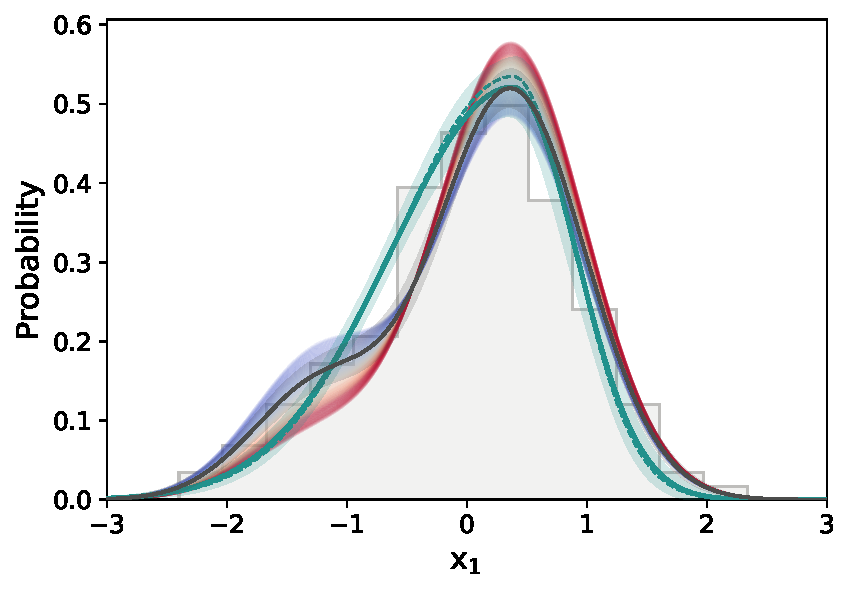
\includegraphics[width=\linewidth]{Article_figures/bbc_comp_PS1_hist-nr.pdf}
    \caption{Distribution of the PS1 SN~Ia \textsc{\texttt{SALT2.4}} stretch
        ($x_1$) after the fiducial redshift limit cut (grey histogram). This
        distribution is supposed to be a random draw from the underlying stretch
        distribution. The green line shows the BBC model of this underlying
        distribution (asymmetric Gaussian). The full line (band) is our best fit
        (its error); the dashed line shows \cite{scolnic2018a} result. The black
        line (band) show our best fitted Base-modeling (its error, see Table
        \ref{tab:modelresults}) that includes redshift drift. For illustration,
        we show as colored (from blue to red with increasing redshifts) the
        evolution of the underlying stretch distribution as a function of
        redshift for the redshift range covered by PS1 data.}
    \label{fig:bbc_pdf_ps1}
\end{figure}

We illustrate in Fig.~\ref{fig:bbc_pdf_ps1} the prediction difference in the
underlying stretch distribution between the BBC modeling and our Base drifting
model for the PS1 sample. Our model is bimodal and the relative amplitude of
each mode depends on the redshift-dependent fraction of old \yc{vs.\ young} SNe~Ia in the
sample: the higher the fraction of old SNe~Ia (at lower redshift), the higher the
amplitude of the \yc{old-specific} low-stretch mode. This redshift dependency is shown as blue to
red underlying distributions in Fig.~\ref{fig:bbc_pdf_ps1} for redshift ranges
covered by PS1. The observed $x_1$ histogram corresponds to the sum of
individual underlying SN-redshift distributions. \yc{Not clear: you mean the black curve -- a model -- or the histogram -- an observation?} As expected, the two approaches \yc{which ones?}
strongly differ in modeling the negative part of the SN stretch distribution.
The BBC asymmetric distribution goes through the middle of the bimodal
distribution, over-estimating the number of SNe~Ia at $x_1\sim-0.7$ and
under-estimating it at $x_1\sim-1.7$ in comparison to our Base drifting
model for typical PS1 SN redshifts. \yc{This is definitely not obvious from the Fig. solely...} This means that the bias-correction of
individual SN stretches, $\overline{\delta}_{x_1}$ \citep{kessler2017}, and
consequently the magnitude bias correction, $\mu_B$, is most likely inaccurate
and \sout{this inaccuracy is} redshift dependent. 

The amplitude of this \yc{magnitude} bias for cosmology is beyond the scope of this paper given
the complexity of the BBC analysis. It would require a full study using our Base
model (Eq.~\ref{eq:stretchz}) in place of the sample-based asymmetric
modeling as part of the BBC simulations.

Nonetheless, it is \yc{enlightening} to study the  expected mean stretch difference as
a function of redshift when considering that the underlying SN stretch
distribution follows either the BBC formalism or our Base drifting model.
This is shown Fig.~\ref{fig:magdrift}, where, for clarity we convert this
difference in \yc{mean??? stretch} $x_1$ to a difference in magnitude using $\alpha=0.156$
\citep{scolnic2018a}.

\begin{figure}
    \centering
    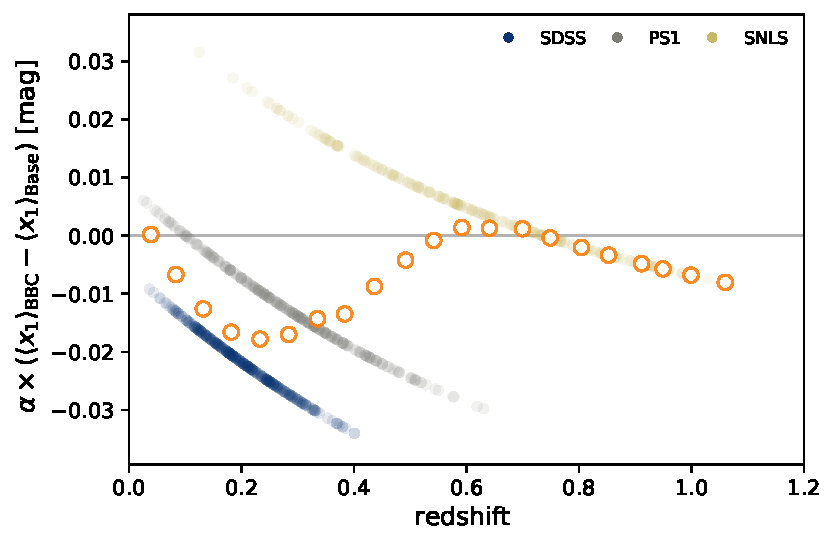
\includegraphics[width=\linewidth]{Article_figures/BBC_-stretchevol_grouped.pdf}
    \caption{Difference of mean stretch standardization (in mag, using
        $\alpha=0.156$ from \citealt{scolnic2018a}) between the BBC algorithm
        and our Base drifting model, as a function of redshift, considering the
        SDSS, PS1 and SNLS datasets. The colored markers show the difference for
        SDSS, PS1 and SNLS samples (see legend) considering the individual SN
    redshifts (no redshift cut applied). The orange markers represent their mean
evolution in 30 regularly-spaced redshift bins.}
    \label{fig:magdrift}
\end{figure}

We see that the amplitude of the modeling difference is a few tens of
millimag, which corresponds to the expected bias affecting SNe~Ia impacted
by sample selection effects. For comparison, the amplitude of this effect is
similar in scale to the effect exotic forms of dark energy could
have on $\mu(z)$. Consequently, in the era of modern cosmology, where we aim at
probing $w_0$ at a sub-percent \yc{level} and $w_a$ at the ten-percent \yc{precision}
\citep[e.g.,][]{lsstpaper}, it is of paramount importance to further
understand the exact modeling of the lightcurve parameters when using SNe~Ia
affected by Malmquist bias.

\section{Conclusion}
\label{sec:ccl}

We have presented a study of the drift of the \yc{intrinsic} SNe~Ia stretch
distribution as a function of redshift. We \yc{built a magnitude-limited SN~Ia sample} from the Pantheon dataset \citep[][SDSS, PS1 and SNLS]{scolnic2018a}, to which we added HST and SNfactory data from \cite{rigault2018} for the
\yc{high- and} low-redshift bins. We only considered the SNe that have been discovered
in the redshift range of each survey where selection effects are negligible, so that the observed SNe~Ia stretches are random sampling of the true underlying
distribution. This \yc{resulted in a} 569 SN~Ia \yc{fiducial sample} (422 SNe when more
conservative cuts were considered).

Following \yc{predictions} made in \cite{rigault2018}, we introduced a redshift
drift model which depends on the expected fraction of ``young'' and ``old'' SNe~Ia as
a function of redshift, each age population having its own \yc{intrinsic} stretch distribution.

In addition to this ``base'' modeling, we have studied various distributions, including \yc{redshift independent} models; we also studied the prediction from the ``Beams
with Bias Correction'', a Malmquist bias correction algorithm used by recent SN~Ia cosmological analyses, \yc{implemented as a} per-sample asymmetric Gaussian distribution.

Our conclusions are the following: \yc{reread and rephrase...}
\begin{enumerate}
    \item Non-drifting models are excluded as good descriptions of the data of
        our Base model. \yc{This does not mean anything...} This model \yc{which one?} assumes that: (1) the younger population has
        a unimodal Gaussian stretch distribution, while the older population
        stretch \yc{distribution} is bimodal, one mode being the same as the young one; (2)
        the evolution of the relative fraction of younger and older SNe~Ia
        follows the prediction made in \cite{rigault2018}. 

    \item Given 1., we conclude that the SNe~Ia stretch is indeed \yc{\sout{drifting} redshift dependent}, as previously suggested by e.g.~\cite{howell2007}. \mr{This result is largely independent of details on each age-population modeling.} \yc{Indeed, and this should be stated first!}

    \item \yc{reread \& rephrase: ``assuming'' is not excluded!} \mr{Assuming survey-based asymmetric
        Gaussian distribution, as done, e.g., in current implementation of the BBC, is excluded to be an as good description of the
        data as our drifting model}. Hence, sample-based approach does not accurately account for redshift drift, unlike what was suggested by
        \cite{scolnic2016} and \cite{scolnic2018a}.

    \item An inaccurate underlying stretch distribution model is estimated to
        bias the mean standardized magnitude of SNe~Ia affected selection
        effects to the order of a few percents. \yc{???} This is comparable in scale to
        the observational signature of exotic forms of dark energy and is
        therefore a significant source of systematic that should be carefully
        studied.

    \item \mr{Given the current dataset}, we suggest the use of the following stretch population model \yc{as a function of redshift}:
        \begin{align}
            \label{eqconclusion:stretchz}
            X_1\left(z \right) =
             &\,\delta(z)\times\mathcal{N}(\mu_1,\sigma_1^2)\,+\nonumber\\
            (1-&\,\delta(z)) \times  \left[a\times\mathcal{N}(\mu_1,\sigma_1^2) +
            (1-a)\times\mathcal{N}(\mu_2,\sigma_2^2)\right]
        \end{align}
    with: $a=0.51$, $\mu_1=0.37$, $\mu_2=-1.22$, $\sigma_1=0.61$,
    $\sigma_2=0.56$ (see Table~\ref{tab:modelresults}) and using the
    age-population drift modelization $\delta(z)$ defined in \cite{rigault2018} \yc{too many R+18 everywhere!}
    with $K=0.87$:
    \begin{align}
        \delta(z) & = \left( K^{-1} \times (1+z)^{-2.8} +1 \right)^{-1}.
    \end{align}
\end{enumerate}

\mr{We considered in this paper a simple Gaussian mixture modeling, but additional data free from
significant Malmquist bias would enable us to refine it. We highlight that samples at the low- and high-redshift ends of the Hubble diagram would be particularly helpful for this drifting analysis; fortunately this will soon be provided by the
Zwicky Transient Facility \citep{bellm2019, graham2019} and Subaru SNe~Ia program (REF HERE ASK NICOLAS), respectively.} 

\begin{acknowledgements}
    This project has received funding from the European Research Council (ERC)
    under the European Union's Horizon 2020 research and innovation programme
    (grant agreement n 759194 - USNAC).
    % How has received that support for this project ? 
    %Support has been provided by the Institut Universitaire de France, the CNES, and the region Auvergne-Rhone-Alpes.
\end{acknowledgements}

\bibliographystyle{aa} % style aa.bst
\begin{thebibliography}{} 
% A
%\bibitem[Abbott et al.(2018)]{abbott2018} Abbott, T.~M.~C., Abdalla, F.~B., Alarcon, A., et al.\ 2018, \prd, 98, 043526

\bibitem[Abbott et al.(2019)]{descosmopaper2019} Abbott, T.~M.~C., Allam, S., Andersen, P., et al.\ 2019, \apjl, 872, L30

\bibitem[Aldering et al.(2002)]{aldering2002} Aldering, G., Adam, G., Antilogus, P., et al.\ 2002, \procspie, 61

\bibitem[Astier et al.(2006)]{astier2006} Astier, P., Guy, J., Regnault, N., et al.\ 2006, \aap, 447, 31


%\bibitem[Ata et al.(2017)]{ata2017} Ata, M., Kitaura, F.-S., Chuang, C.-H., et al.\ 2017, \mnras, 467, 3993

\bibitem[Aubourg et al.(2008)]{aubourg2008} Aubourg, {\'E}.,
  Tojeiro, R., Jimenez, R., et al.\ 2008, \aap, 492, 631 


% B
\bibitem[Bazin et al.(2011)]{bazin2011} Bazin, G., Ruhlmann-Kleider, V., Palanque-Delabrouille, N., et al.\ 2011, \aap, 534, A43

\bibitem[Bellm et al.(2019)]{bellm2019} Bellm, E.~C., Kulkarni, S.~R., Graham, M.~J., et al.\ 2019, \pasp, 131, 018002

\bibitem[Betoule et al.(2014)]{betoule2014} Betoule, M., Kessler, R., Guy, J., et al.\ 2014, \aap, 568, A22

\bibitem[Brout et al.(2019)]{brout2019} Brout, D., Scolnic, D., Kessler, R., et al.\ 2019, \apj, 874, 150

\bibitem[Burnham \& Anderson(2004)]{burnham2004} Burnham, K., Anderson, D., \
2004, Sociological Methods \& Research, 33, 2

% C
\bibitem[Campbell et al.(2013)]{campbell2013} Campbell, H., D'Andrea, C.~B., Nichol, R.~C., et al.\ 2013, \apj, 763, 88


%\bibitem[Chabanier et al.(2019)]{chabanier2019} Chabanier, S., Millea, M., \& Palanque-Delabrouille, N.\ 2019, \mnras, 489, 2247

\bibitem[Childress et al.(2013)]{childress2013} Childress, M., Aldering, G., Antilogus, P., et al.\ 2013, \apj, 770, 108

\bibitem[Childress et al.(2014)]{childress2014} Childress, M.~J., Wolf, C., \& Zahid, H.~J.\ 2014, \mnras, 445, 1898


%\bibitem[Coles, \& Jones(1991)]{coles1991} Coles, P., \& Jones, B.\ 1991, \mnras, 248, 1

%\bibitem[Conley et al.(2011)]{conley2011} Conley, A., Guy, J., Sullivan, M., et al.\ 2011, \apjs, 192, 1


% D
\bibitem[D'Andrea et al.(2011)]{dandrea2011} D'Andrea, C.~B., Gupta, R.~R., Sako, M., et al.\ 2011, \apj, 743, 172

\bibitem[Dilday et al.(2008)]{dilday2008} Dilday, B., Kessler, R., Frieman, J.~A., et al.\ 2008, \apj, 682, 262


% E
% F
\bibitem[Feeney et al.(2019)]{feeney2019} Feeney, S.~M., Peiris, H.~V., Williamson, A.~R., et al.\ 2019, \prl, 122, 061105

\bibitem[Freedman et al.(2019)]{freedman2019} Freedman, W.~L., Madore, B.~F., Hatt, D., et al.\ 2019, \apj, 882, 34

\bibitem[Freedman et al.(2020)]{freedman2020} Freedman, W.~L., Madore, B.~F., Hoyt, T., et al.\ 2020, arXiv e-prints, arXiv:2002.01550



\bibitem[Frieman et al.(2008)]{frieman2008} Frieman, J.~A., Bassett, B., Becker, A., et al.\ 2008, \aj, 135, 338


% G
\bibitem[Graham et al.(2019)]{graham2019} Graham, M.~J., Kulkarni, S.~R., Bellm, E.~C., et al.\ 2019, \pasp, 131, 078001

\bibitem[Gupta et al.(2011)]{gupta2011} Gupta, R.~R., D'Andrea, C.~B., Sako, M., et al.\ 2011, \apj, 740, 92

\bibitem[Guy et al.(2007)]{guy2007} Guy, J., Astier, P., Baumont, S., et al.\ 2007, \aap, 466, 11

%\bibitem[Guy et al.(2010)]{guy2010} Guy, J., Sullivan, M., Conley, A., et al.\ 2010, \aap, 523, A7

%\bibitem[Graziani et al.(2019)]{graziani2019} Graziani, R., Courtois, H.~M., Lavaux, G., et al.\ 2019, \mnras, 488, 5438

% H
\bibitem[Hamuy et al.(1996)]{hamuy1996} Hamuy, M., Phillips, M.~M., Suntzeff, N.~B., et al.\ 1996, \aj, 112, 2391

\bibitem[Hamuy et al.(2000)]{hamuy2000} Hamuy, M., Trager, S.~C., Pinto, P.~A., et al.\ 2000, \aj, 120, 1479

\bibitem[Hinton et al.(2019)]{hinton2019} Hinton, S.~R., Davis, T.~M., Kim, A.~G., et al.\ 2019, \apj, 876, 15


\bibitem[Howell et al.(2007)]{howell2007} Howell, D.~A., Sullivan, M., Conley, A., et al.\ 2007, \apjl, 667, L37

%\bibitem[Howell et al.(2009)]{howell2009} Howell, D.~A., Sullivan, M., Brown, E.~F., et al.\ 2009, \apj, 691, 661

% I
\bibitem[Ivezi{\'c} et al.(2019)]{lsstpaper} Ivezi{\'c}, {\v{Z}}., Kahn, S.~M., Tyson, J.~A., et al.\ 2019, \apj, 873, 111


% J
\bibitem[Jones et al.(2015)]{jones2015} Jones, D.~O., Riess, A.~G., \& Scolnic, D.~M.\ 2015, \apj, 812, 3
1

\bibitem[Jones et al.(2018)]{jones2018} Jones, D.~O., Riess, A.~G., Scolnic, D.~M., et al.\ 2018, \apj, 867, 108

\bibitem[Jones et al.(2018)b]{jones2018b} Jones, D.~O., Scolnic, D.~M., Riess, A.~G., et al.\ 2018, \apj, 857, 51

\bibitem[Jones et al.(2019)]{jones2019} Jones, D.~O., Scolnic, D.~M., Foley, R.~J., et al.\ 2019, \apj, 881, 19

% K
\bibitem[Kelly et al.(2010)]{kelly2010} Kelly, P.~L., Hicken, M., Burke, D.~L., et al.\ 2010, \apj, 715, 743

\bibitem[Kessler et al.(2009)]{kessler2009} Kessler, R., Becker, A.~C., Cinabro, D., et al.\ 2009, \apjs, 185, 32

\bibitem[Kessler \& Scolnic(2017)]{kessler2017} Kessler, R., \& Scolnic, D.\ 2017, \apj, 836, 56

\bibitem[Kim et al.(2018)]{kim18} Kim, Y.-L., Smith, M., Sullivan, M., et al.\ 2018, \apj, 854, 24

\bibitem[Kim et al.(2019)]{kim19} Kim, Y.-L., Kang, Y., \& Lee, Y.-W.\ 2019, Journal of Korean Astronomical Society, 52, 181

\bibitem[Knox \& Millea(2019)]{knox2019} Knox, L., \& Millea, M.\ 2019, arXiv e-prints, arXiv:1908.03663

% L
\bibitem[Lampeitl et al.(2010)]{lampeitl2010} Lampeitl, H., Smith, M., Nichol, R.~C., et al.\ 2010, \apj, 722, 566

% M
\bibitem[Mannucci et al.(2005)]{mannucci2005} Mannucci, F.,
  Della Valle, M., Panagia, N., et al.\ 2005, \aap, 433, 807 
\bibitem[Mannucci et al.(2006)]{mannucci2006} Mannucci, F.,
  Della Valle, M., \& Panagia, N.\ 2006, \mnras, 370, 773 

\bibitem[Maoz et al.(2014)]{maozmannucci2014} Maoz, D., Mannucci,
  F., \& Nelemans, G.\ 2014, \araa, 52, 107 


% N
\bibitem[Neill et al.(2006)]{neill2006} Neill, J.~D., Sullivan, M., Balam, D., et al.\ 2006, \aj, 132, 1126

\bibitem[Neill et al.(2009)]{neill2009} Neill, J.~D., Sullivan, M., Howell, D.~A., et al.\ 2009, \apj, 707, 1449

% O
% P
\bibitem[Pan et al.(2014)]{pan2014} Pan, Y.-C., Sullivan, M., Maguire, K., et al.\ 2014, \mnras, 438, 1391

\bibitem[Perlmutter et al.(1999)]{perlmutter1999} Perlmutter, S., Aldering, G., Goldhaber, G., et al.\ 1999, \apj, 517, 565

\bibitem[Perrett et al.(2010)]{perrett2010} Perrett, K., Balam, D., Sullivan, M., et al.\ 2010, \aj, 140, 518

%\bibitem[Planck Collaboration et al.(2016)]{planck2016} Planck Collaboration, Ade, P.~A.~R., Aghanim, N., et al.\ 2016, \aap, 594, A13


\bibitem[Planck Collaboration et al.(2018)]{planck2018} Planck Collaboration, Aghanim, N., Akrami, Y., et al.\ 2018, arXiv e-prints, arXiv:1807.06209

\bibitem[Poulin et al.(2019)]{poulin2019} Poulin, V., Smith, T.~L., Karwal, T., et al.\ 2019, \prl, 122, 221301

% Q
% R
\bibitem[Reid et al.(2019)]{reid2019} Reid, M.~J., Pesce, D.~W., \& Riess, A.~G.\ 2019, arXiv e-prints, arXiv:1908.05625

\bibitem[Rest et al.(2014)]{rest2014} Rest, A., Scolnic, D., Foley, R.~J., et al.\ 2014, \apj, 795, 44

\bibitem[Riess et al.(1998)]{riess1998} Riess, A.~G., Filippenko, A.~V., Challis, P., et al.\ 1998, \aj, 116, 1009

\bibitem[Riess et al.(2009)]{riess2009} Riess, A.~G., Macri, L., Casertano, S., et al.\ 2009, \apj, 699, 539

\bibitem[Riess et al.(2016)]{riess2016} Riess, A.~G., Macri, L.~M., Hoffmann, S.~L., et al.\ 2016, \apj, 826, 56

\bibitem[Riess et al.(2018)]{riess2018} Riess, A.~G., Casertano, S., Yuan, W., et al.\ 2018, \apj, 861, 126

\bibitem[Riess et al.(2019)]{riess2019} Riess, A.~G., Casertano, S., Yuan, W., et al.\ 2019, \apj, 876, 85

\bibitem[{Rigault {et~al.}(2013)}]{rigault2013}
Rigault, M., Copin, Y., Aldering, G., {et~al.} 2013, \aap, 560, A66

\bibitem[Rigault et al.(2015)]{rigault2015} Rigault, M., Aldering, G., Kowalski, M., et al.\ 2015, \apj, 802, 20

\bibitem[Rigault et al.(2018)]{rigault2018} Rigault, M.,
  Brinnel, V., Aldering, G., et al.\ 2018, arXiv:1806.03849

\bibitem[Rodney et al.(2014)]{rodney2014} Rodney, S.~A.,
  Riess, A.~G., Strolger, L.-G., et al.\ 2014, \aj, 148, 13 
  
\bibitem[Roman et al.(2018)]{roman2018} Roman, M., Hardin, D., Betoule, M., et al.\ 2018, \aap, 615, A68

\bibitem[Rose et al.(2019)]{rose2019} Rose, B.~M., Garnavich, P.~M., \& Berg, M.~A.\ 2019, \apj, 874, 32


\bibitem[Rubin et al.(2015)]{rubin2015} Rubin, D., Aldering, G., Barbary, K., et al.\ 2015, \apj, 813, 137

\bibitem[Rubin \& Hayden(2016)]{rubin2016} Rubin, D., \& Hayden, B.\ 2016, \apjl, 833, L30


% S
\bibitem[Sako et al.(2008)]{sako2008} Sako, M., Bassett, B., Becker, A., et al.\ 2008, \aj, 135, 348

\bibitem[Scannapieco \& Bildsten(2005)]{scannapieco2005} Scannapieco, E., \& Bildsten, L.\ 2005, \apjl, 629, L85 

\bibitem[Scolnic et al.(2014)]{scolnic2014} Scolnic, D., Rest, A., Riess, A., et al.\ 2014, \apj, 795, 45

\bibitem[Scolnic \& Kessler(2016)]{scolnic2016} Scolnic, D., \& Kessler, R.\ 2016, \apjl, 822, L35


\bibitem[Scolnic et al.(2018)]{scolnic2018a} Scolnic, D.~M., Jones, D.~O., Rest, A., et al.\ 2018a, \apj, 859, 101

%\bibitem[Scolnic et al.(2018)]{scolnic2018b} Scolnic, D.~M., Lochner, M., Gris, P., et al.\ 2018, arXiv e-prints, arXiv:1812.00516

\bibitem[Scolnic et al.(2019)]{scolnicastro2020} Scolnic, D., Perlmutter, S., Aldering, G., et al.\ 2019, Astro2020: Decadal Survey on Astronomy and Astrophysics, 2020, 270

\bibitem[Shariff et al.(2016)]{shariff2016} Shariff, H., Jiao, X., Trotta, R., et al.\ 2016, \apj, 827, 1


\bibitem[Strolger et al.(2004)]{strolger04} Strolger, L.-G., Riess, A.~G., Dahlen, T., et al.\ 2004, \apj, 613, 200

\bibitem[Sullivan et al.(2006)]{sullivan2006} Sullivan, M., Le  Borgne, D., Pritchet, C.~J., et al.\ 2006, \apj, 648, 868 


\bibitem[Sullivan et al.(2010)]{sullivan2010} Sullivan, M., Conley, A., Howell, D.~A., et al.\ 2010, \mnras, 406, 782

% T
\bibitem[Tasca et al.(2015)]{tasca2015} Tasca, L.~A.~M., Le F{\`e}vre, O., Hathi, N.~P., et al.\ 2015, \aap, 581, A54

% U 
% V
% W
\bibitem[Wiseman et al.(2020)]{wiseman2020} Wiseman, P., Smith, M., Childress, M., et al.\ 2020, arXiv e-prints, arXiv:2001.02640


\bibitem[Wong et al.(2019)]{wong2019} Wong, K.~C., Suyu, S.~H., Chen, G.~C.-F., et al.\ 2019, arXiv e-prints, arXiv:1907.04869

% X
% Y

% Z
\end{thebibliography}
\end{document}


%%%%%%%%%%%%%%%%%%%%%%%%
%
%  BACKUP 
%
%%%%%%%%%%%%%%%%%%%%%%%%


%For clarity with the next models, we named it 3G2M2S$_{\text{SNf}}$ for it has a total of 3 gaussians but with only 2 means and 2 standard deviations, and has been fitted on SNf data only. 

%We implemented and compared 10 models in total, 4 of which have an
%evolution with the redshift from $\delta(z)$, and 6 don't ($\delta(z) = f =\mathrm{cst}$). The ones with and evolution are:
\begin{itemize}
    \item 3G2M2S, the one we described (but fitted on all the data);
    \item 3G2M1S, where this time $\sigma_1 \equiv \sigma_2$;
    \item 2G2M2S, model taken from HOWELL 2009 where we added $\delta(z)$;
    \item 3G3M3S, with three independent gaussians.
\end{itemize}
The ones without a stretch evolution are the same ones but with an ``F'' implying
we set $\delta(z) = f = \mathrm{cst}$, and two others:
\begin{itemize}
    \item 1G1M1S, where there is no distinction between old and young SNe;
    \item 1G1M2S, taken from KESLLER 2017 and used in recent cosmological
        analysis SCOLNIC 2018. It's an asymetric model where
\end{itemize}
\begin{align}
 p(x_1^i, \mathrm{d} x_1^i | \mu, \sigma_-, \sigma_+) = 
    \begin{cases}
        \mathcal{N} \left(\mu, \sqrt{\sigma_-{}^2 + \mathrm{d} x_1^i{}^{2}}\right) (x_1^i) & \text{if
        } x_1^i\geq \mu\\
        \mathcal{N} \left(\mu, \sqrt{\sigma_+{}^2 + \mathrm{d} x_1^i{}^{2}}\right) (x_1^i), &
        \text{else}
    \end{cases}
\end{align} 

The fitted parameters are shown in Table~\ref{tab:val}.

\begin{table*}[htbp!]
    \centering
    \caption{Values of the best-it parameters for all the models. In red are the non-coherent ones which coincides with the models without an evolution of the fraction of young SNe Ia with the redshift.}
    \label{tab:val}
    \begin{tabular}{c c c c c c c}\hline\hline

        Model & $a$ & $f$ & $\mu_1$ & $\sigma_1$ & $\mu_2$ &
        $\sigma_2$ \\\hline

        3G2M2S$_{\mathrm{SNf}}$ & $0.48 \pm 0.07$ & none & $0.39 \pm 0.07$ &
        $0.56 \pm 0.05$ & $-1.5 \pm 0.1$ & $0.52 \pm 0.09$ \\

        3G2M2S & $0.48 \pm 0.17$ & none & $0.36 \pm 0.08$ & $0.61 \pm 0.05$ &
        $-1.3 \pm 0.2$ & $0.60 \pm 0.12$ \\

        3G2M2SF & \textcolor{red}{$0.1 \pm 0.6$} & \textcolor{red}{$0.2 \pm
        0.6$} & $-0.9 \pm 0.7$ & $0.7 \pm 0.3$ & $0.5 \pm 0.2$ & $0.6 \pm 0.1$
        \\

        3G2M1S & $0.47 \pm 0.07$ & none & $0.35 \pm 0.04$ & $0.61 \pm 0.03$ &
        $-1.25 \pm 0.10$ & $\sigma_1$ \\

        3G2M1SF & \textcolor{red}{$0.2 \pm 0.9$} & $0.7 \pm 0.3$ & $0.36 \pm
        0.04$ & $0.60 \pm 0.03$ & $-1.23 \pm 0.10$ & $\sigma_1$ \\

        2G2M2S & none & none & $0.49 \pm 0.04$ & $0.54 \pm 0.03$ & $-0.72 \pm
        0.08$ & $0.83 \pm 0.07$ \\
        
        2G2M2SF & none & $0.3 \pm 0.2$ & $-0.9 \pm 0.6$ & $0.7 \pm 0.2$ & $0.5
        \pm 0.2$ & $0.56 \pm 0.09$ \\\hline

    \end{tabular} \bigbreak

\begin{tabular}{c c c}\hline\hline

    Model & $\mu$ & $\sigma$ \\\hline

    1G1M1S & $0.01 \pm 0.04$ & $0.90 \pm 0.03$ \\\hline

\end{tabular} \bigbreak

\begin{tabular}{c c c c c}\hline\hline

    Model & $\mu$ & $\sigma_-$ & $\sigma_+$ \\\hline

    1G1M2S & $0.16617 \pm 0.00004$ & $1.07 \pm 0.04$ & $0.69 \pm 0.03$ \\\hline

\end{tabular} \bigbreak

\begin{tabular}{c c c c c c c c c}\hline\hline

    Model & $a$ & $f$ & $\mu_1$ & $\sigma_1$ & $\mu_2$ & $\sigma_2$ &
    $\mu_3$ & $\sigma_3$ \\\hline

    3G3M3S & $0.14 \pm 0.08$ & none & $0.51 \pm 0.06$ & $0.54 \pm 0.04$ & $-1.9
    \pm 0.2$ & $0.29 \pm 0.11$ & $-0.55 \pm 0.12$ & $0.67 \pm 0.15$ \\
    
    3G3M3SF & $0.2 \pm 0.2 $ & $0.10 \pm 0.04 $ & $-1.7 \pm 0.2$ & $0.4 \pm 0.1$
            & $0.9 \pm 0.1$ & $0.3 \pm 0.2$ & $0.0 \pm 0.2$ & $0.7 \pm 0.1$
            \\\hline

\end{tabular} \bigbreak
\end{table*}

To test the coherence of this model, we also fitted it using all the data from
the surveys indistinctly. These results are shown Fig.~\ref{fig:model_all}.

\begin{table*}
    \centering
    \caption{BBC comparison}
    \label{tab:bbc_comp}
    \begin{tabular}{c c |c c c |c c c |c c c}\hline\hline\\[-1.05em]
     &  & \multicolumn{3}{|c}{Asym (this)} & \multicolumn{3}{|c}{Asym (SK18/S18)} & \multicolumn{3}{|c}{Base SNf} \\
    N$_{\mathrm{SN}}$ & Survey & $\mathcal{X}^2$ & AIC & Free param & $\mathcal{X}^2$ & AIC & Free param & $\mathcal{X}^2$ & AIC & Free param \\\hline
    167 & SDSS & 445.0 & 451.2 & 3 & 457.9 & 464.0 & 3 & 452.9 & 452.9 & 0\\
    160 & PS1 & 397.4 & 403.6 & 3 & 397.6 & 403.7 & 3 & 405.2 & 405.2 & 0\\
    102 & SNLS & 252.7 & 259.0 & 3 & 254.5 & 260.8 & 3 & 269.5 & 269.5 & 0\\
    114 & SNf & 299.3 & 305.5 & 3 & -- & -- & -- & 268.6 & 279.1 & 5\\
    543 & Total & 1394.5 & 1419.1 & 12 & -- & -- & -- & 1396.0 & 1406.2 & 5\\
    429 & Total-SNf & 1095.2 & 1113.6 & 9 & 1110.0 & 1128.4 & 9 & 1127.5 & 1127.5 & 0\\\hline\hline
    \end{tabular}
\end{table*}

\begin{table*}
    \centering
    \caption{BBC comparison}
    \label{tab:bbc_comp}
    \begin{tabular}{c |c c c |c c c}\hline\hline\\[-1.05em]
     & \multicolumn{3}{|c}{Asym (this)}  & \multicolumn{3}{|c}{Base SNf} \\
    Survey & $\mathcal{X}^2$ & AIC & Free param & $\mathcal{X}^2$ & AIC & Free param \\\hline
    SNf & 299.3 & 305.5 & 3 & 268.6 & 279.1 & 5\\
    SDSS & 445.0 & 451.2 & 3 & 452.9 & 452.9 & 0\\
    PS1 & 397.4 & 403.6 & 3 & 405.2 & 405.2 & 0\\
    SNLS & 252.7 & 259.0 & 3  & 269.5 & 269.5 & 0\\
    Total & 1394.5 & 1419.1 & 12 & 1396.0 & 1406.2 & 5\\\hline\hline
    \end{tabular}
\end{table*}we are also testing non-drifting models by restricting the ``Base'' and ``Howell'' models to use a supposedly redshift-independent fraction $\delta(z) = f$ of young SNe; these models are labeled ``Base constant'' and ``Howell constant''.} \yc{\uline{fix labels!!! \nn{done}}}

